\section{Dataset}

Whilst \gls{mammographic images} are the dataset of choice, this project could be applied to any grey-scale image set, such as other medical imagery. The choice to use \gls{mammographic images} was a personal one due to family history and an interest in aiding medicine via computer science techniques.

There exists several publically-available, anonymised mammographic datasets, so there was no issues in obtaining data without ethical concerns. The ethics form completed for the University can be found in Appendix \ref{appendix:ethics}. This section will outline the main open datasets considered for this project.

\subsection{Mammographic Image Analysis Society (MIAS) database}

The chosen dataset is a version of the \acrfull{MIAS}'s database, as it is commonly used within the research field and compiled for the sole purpose of trying to better understand mammograms. The original \acrshort{MIAS} database has been refined to create the mini-\acrshort{MIAS} database which contains the same data, however with a size of 1024x1024 pixels. This size is preferable over the original \acrshort{MIAS} data, as it is a lot quicker to process.

Examples of mini-\acrshort{MIAS} images can be found throughout the document, however for reference, an example can be seen in Figure \ref{fig:mini-mias}

\begin{figure}[H]
  \centering
  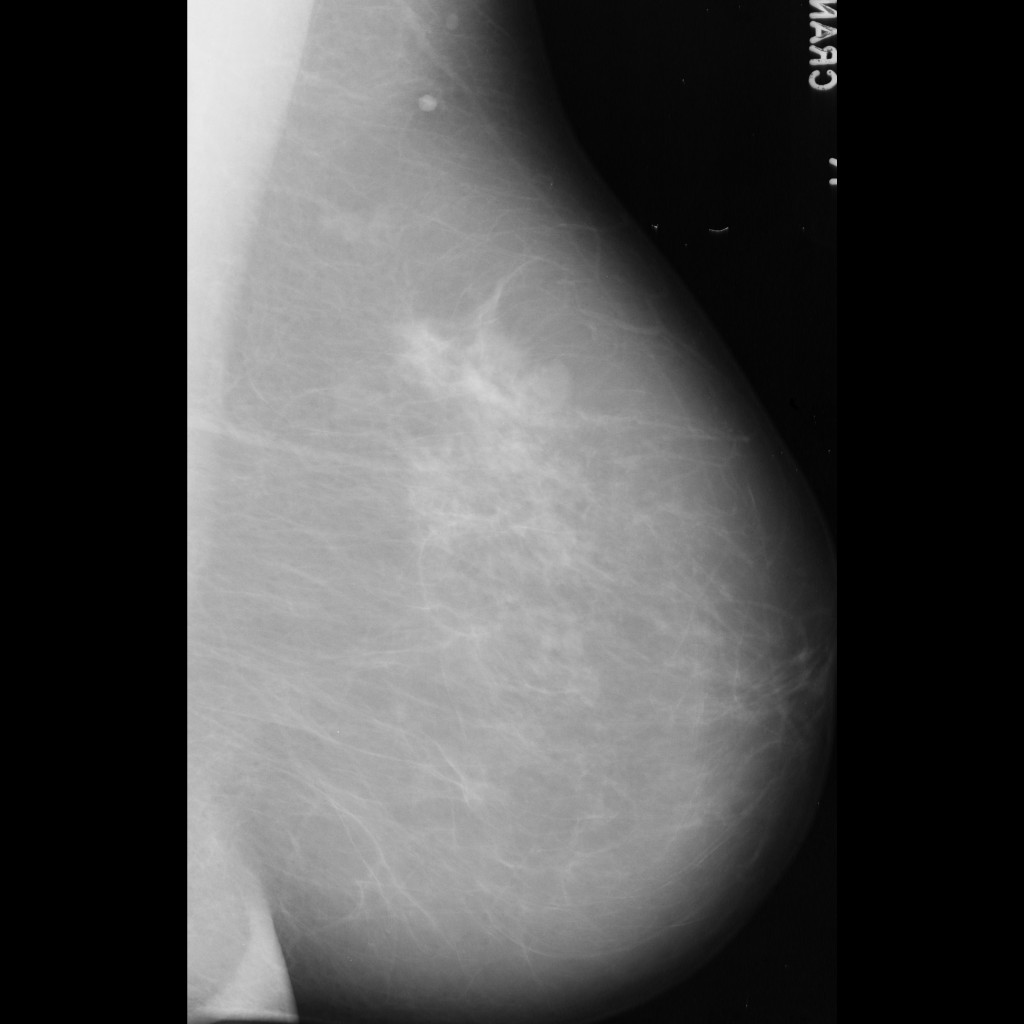
\includegraphics[width=0.4\textwidth]{Chapter2/tools/mias.jpg}
  \caption{Example mini-MIAS scan, scaled down for inclusion in document.}
  \label{fig:mini-mias}
\end{figure}

\subsection{Other datasets}

\noindent \textbf{Digital Database for Screening Mammography (DDSM)}

The \acrshort{DDSM} database was created after a collobration between Massachusetts General Hospital, Sandia National Laboratories and the University of South Florida Computer Science and Engineering Department and contains around 2,500 images \cite{Heath_Bowyer_Kopans_Moore_Kegelmeyer_Processing} \cite{Heath_Bowyer_Kopans_Kegelmeyer_Moore_Chang_MunishKumaran_1998}.
However, like the original \acrshort{MIAS} database, the images available via the acrshort{DDSM} are extremely large, and therefore unsuitable for this project due to the time it would take to process.

\noindent \textbf{Mammographic Mass Data Set}

As the name suggests, this dataset contains 961 instances of scans containing masses - both benign and malignant \cite{Elter_Schulz-Wendtland_Wittenberg_2007}. This project aims to work with solely healthy tissue, therefore this dataset is not beneficial.
